\documentclass[10pt]{ctexart}
\usepackage{graphicx, amsmath}
\usepackage{siunitx}
\usepackage{caption}
\usepackage[version=4]{mhchem}
\title{康普顿散射实验}
\author{张爱强\\指导教师: 张钊}
\date{}
% set the section title format
\ctexset{
    section/format  += \raggedright
}
% The following parameters seem to provide a reasonable page setup.
\topmargin 0.0cm
\oddsidemargin 0.2cm
\textwidth 16cm 
\textheight 21cm
\footskip 1.0cm
% set the abstract format
\newenvironment{sciabstract}{%
\begin{quote} \textbf{摘要: }}
{\end{quote}}
% set the bibliography format
\bibliographystyle{elsarticle-num}


\begin{document}
\maketitle
\begin{sciabstract}
    本实验使用塑料闪烁体和\ce{NaI}闪烁体符合测量康普顿微分散射截面和散射角的关系。利用\ce{^{57}Co}放射源衰变后准直的$\gamma$入射进入塑料闪烁体,
    发生康普顿效应,利用\ce{NaI}闪烁体测量散射光子能谱。调整不同的角度,得到散射角和微分散射截面之间的关系。
    \par\textbf{关键词: } 康普顿散射; 符合方法.
\end{sciabstract}
\section{引言}
康普顿散射验证光的粒子性,该研究在1927年获Nobel Prize。

$\gamma$光子能量比外层电子的结合能大的多,可以把外层电子看作自由电子。利用动量能量守恒可以获得散射$\gamma$光子和散射角的关系。散射$\gamma$光子能量
\[\]
用Dirac方程可以得到计算康普顿散射的微分截面的Klein-Nishna公式:
\[\]
\section{实验}
\subsection{实验仪器}
\begin{description}
    \item[放射源铅室] 内部有放射源,射线从准直器出射,保证射线方向。后侧有一个旋钮,旋转180\si{degree}控制准直器出口的打开与关闭。 
    \item[\ce{NaI(Tl)}闪烁体] 测量散射光子的能谱
    \item[符合器件] 对两路信号进行符合。
\end{description}

\subsection{实验内容}
\begin{enumerate}
    \item 在散射角$\theta=60^\circ$,用\ce{^{137}Cs},\ce{^{60}Co}对探测器\ce{NaI}进行能量刻度。
    \item 在不同散射角分别用符合法测量\ce{^{137}Cs}的$\gamma$能谱,定出全能峰总计数
    \item 求不同$\theta$的散射$\gamma$能量以及散射微分截面的相对值。
\end{enumerate}
\section{实验结果及讨论}
\subsection{能量刻度}
用多道直接测量\ce{NaI(Tl)}闪烁体探测器输出的能谱为图~\ref{fig:EnergyPeakFix}。\ce{^{137}Cs},\ce{^{60}Co}对应于三个特征峰,分别为
\SI{0.662}{MeV},\SI{1.1732}{MeV},\SI{1.3325}{MeV}。从道址90到300之间寻峰,可以排除掉前面的低能本底和后面大部分无用的能量区间,其次
寻找峰位满足大于左右两侧4个道址,而且距左边10个道址处的幅度要下降为峰值的2/3,筛选出如图~\ref{fig:EnergyPeakFix}中黑色三角形指示的三个位置。
将这三个道址和对应的能量使用线性函数拟合。
\begin{figure}[htbp]
    \centering
    \begin{minipage}{0.45\textwidth}
        \centering
        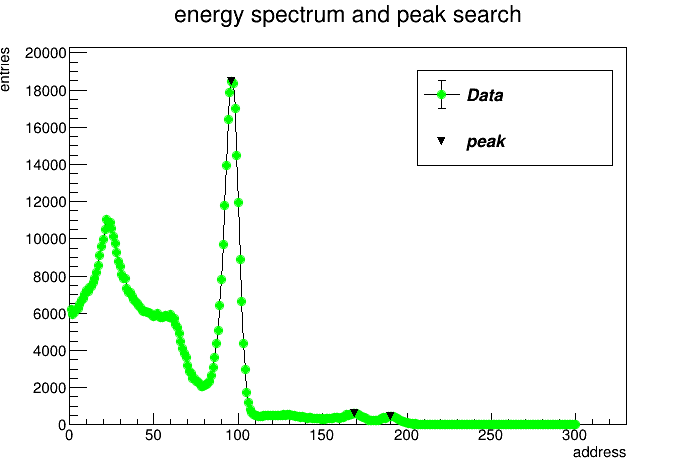
\includegraphics[width=\textwidth]{data/scaleEnergy.png}
        \caption{寻峰}
        \label{fig:EnergyPeakFix}
    \end{minipage}
    \qquad
    \begin{minipage}{0.45\textwidth}
        \centering
        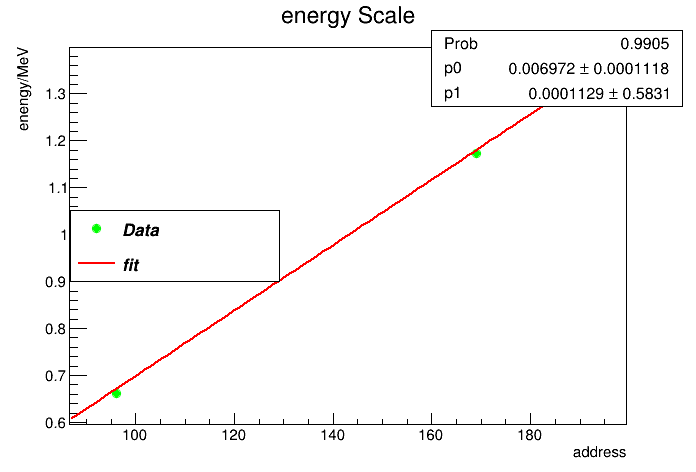
\includegraphics[width=\textwidth]{data/scaleEnergyFit.png}
        \caption{能量刻度}
        \label{fig:EnergyFix}
    \end{minipage}
\end{figure}
图~\ref{fig:EnergyFix}三个特殊的峰的位置对应的道址分别为$18,76,$,利用线性函数进行刻度,拟合得到道址和能量之间的关系。
\[E(MeV)=(0.00697\pm 0.00011)x+(0\pm 0.58)\]
\subsection{探测效率和峰总比与能量的关系}
使用多项式进行插值,为了避免过拟合,设置多项式最大阶数为4,拟合对应的插值函数。
\begin{figure}[htbp]
    \centering
    \begin{minipage}{0.45\textwidth}
        \centering
        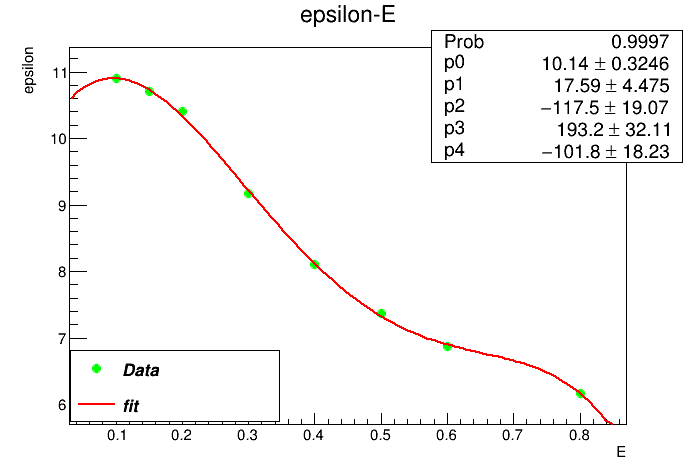
\includegraphics[width=\textwidth]{data/epsilon.png}
        \caption{探测效率和能量}
        \label{fig:epsilon}
    \end{minipage}
    \qquad
    \begin{minipage}{0.45\textwidth}
        \centering
        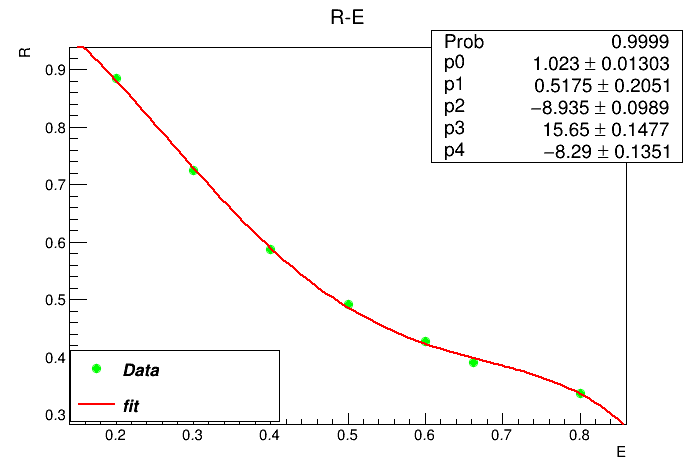
\includegraphics[width=\textwidth]{data/R.png}
        \caption{峰总比和能量}
        \label{fig:R}
    \end{minipage}
\end{figure}
图~\ref{fig:epsion}和图~\ref{fig:R}利用线性函数进行刻度,拟合得到探测效率和峰总比与能量之间的关系。
\[\epsilon=(10.13\pm0.32)+(17.58\pm 4.47)x+(-117.5\pm19.1)x^2+(193.2\pm32.1)x^3+(-101.8\pm18.2)x^4\]
\[R=(1.023\pm0.013)+(0.52\pm 0.21)x+(-8.935\pm0.099)x^2+(15.65\pm0.15)x^3+(-8.29\pm0.14)x^4\]
\subsection{康普顿散射光子能量拟合}
通过寻峰和能量刻度结果可以获得不同$\theta$下对应的道址和能量如图~\ref{fig:theta20}等和表\ref{tab:gammaEnergy}.

\begin{figure}
    \centering
    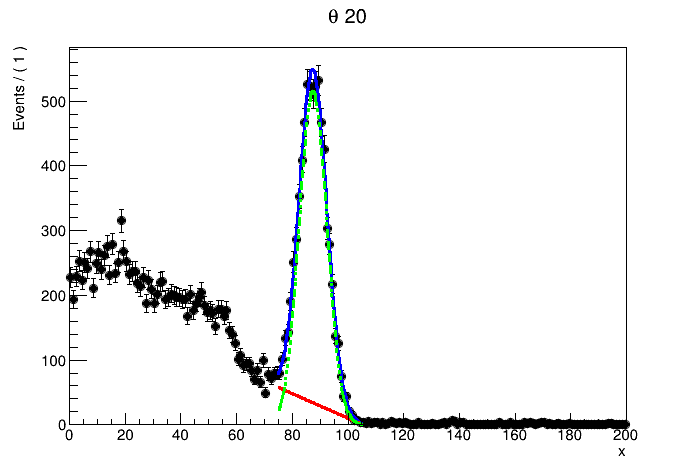
\includegraphics[width=0.6\textwidth]{data/20.png}
    \caption{$\theta=20^\circ$}
    \label{fig:theta20}
\end{figure}
\begin{figure}
    \centering
    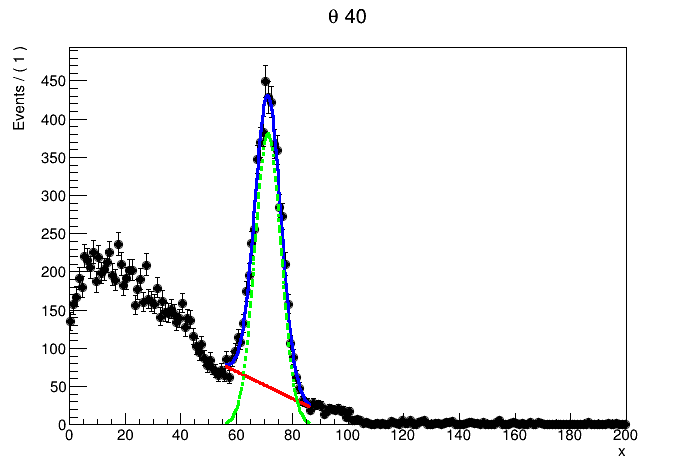
\includegraphics[width=0.6\textwidth]{data/40.png}
    \caption{$\theta=40^\circ$}
    \label{fig:theta40}
\end{figure}
\begin{figure}
    \centering
    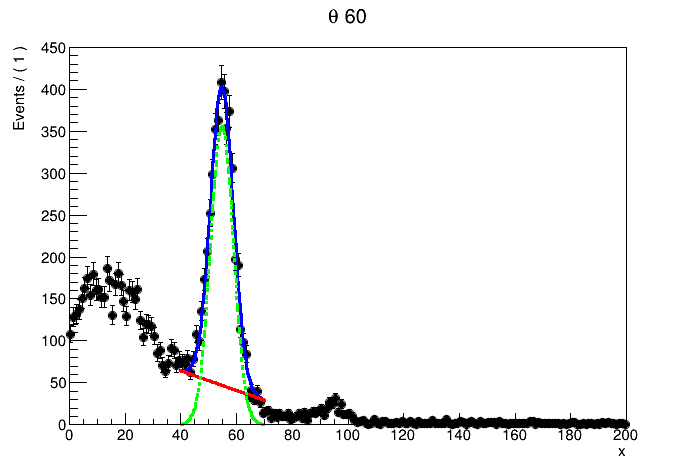
\includegraphics[width=0.6\textwidth]{data/60.png}
    \caption{$\theta=60^\circ$}
    \label{fig:theta60}
\end{figure}
\begin{figure}
    \centering
    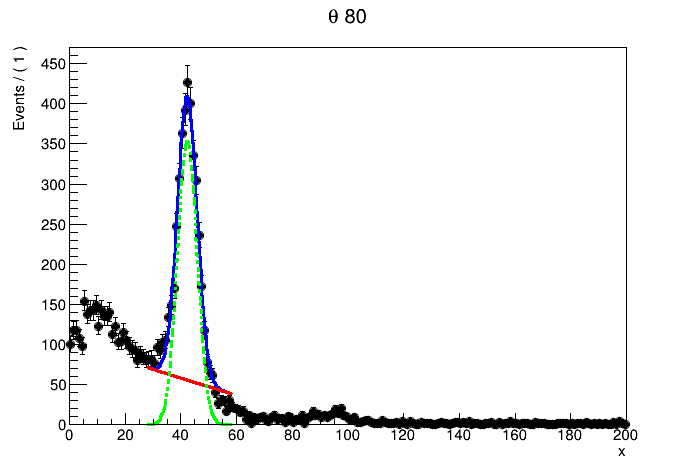
\includegraphics[width=0.6\textwidth]{data/80.png}
    \caption{$\theta=80^\circ$}
    \label{fig:theta80}
\end{figure}
\begin{figure}
    \centering
    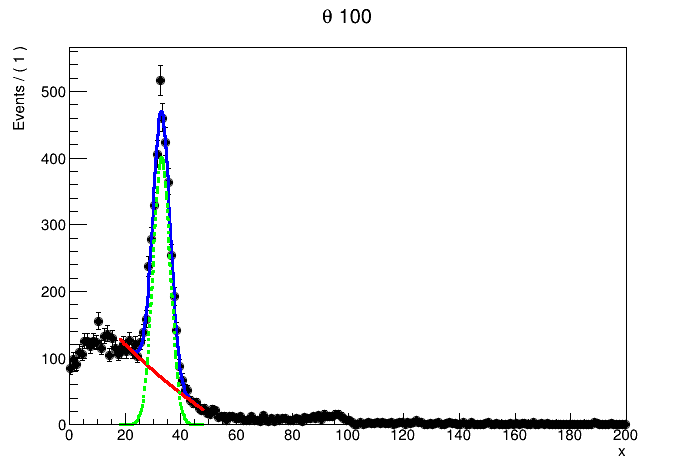
\includegraphics[width=0.6\textwidth]{data/100.png}
    \caption{$\theta=100^\circ$}
    \label{fig:theta100}
\end{figure}
\begin{figure}
    \centering
    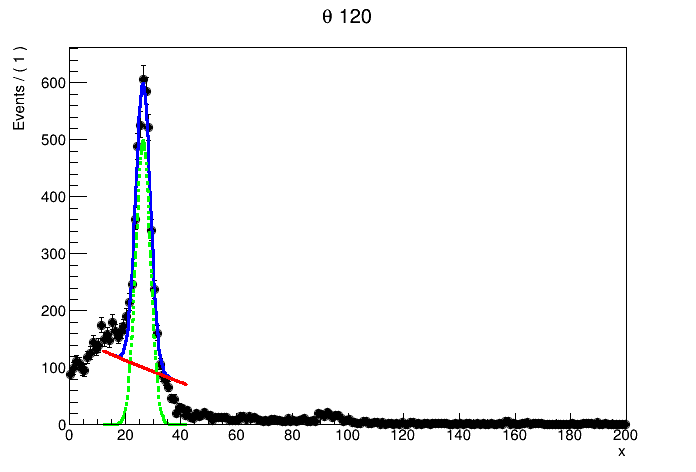
\includegraphics[width=0.6\textwidth]{data/120.png}
    \caption{$\theta=120^\circ$}
    \label{fig:theta120}
\end{figure}
因为探测器会有一个能量分辨率,所以全能峰对应于一个高斯分布;另外由于本底的存在,全能峰对应部分有一个本底的叠加。利用高斯和二次函数本底\cite{}叠加拟合得到
拟合结果分别如图~\ref{fig:theta40}等,对应的全能峰计数标记在表\ref{tab:gammaEnergy}

\begin{table}
    \begin{tabular}{|c|c|c|c|}
        \textbf{$\theta$} & \textbf{道址}& \textbf{全能峰计数}& \textbf{$E_{\gamma}$}& \textbf{全能峰计数}\\
        \hline
                 20   &87.455606 & 6355.6201 &0.610\\
                40 & 71.267048 & 4483.3065 &0.497\\
                60 & 54.747531 & 3653.1918 &0.382\\
                80 & 42.312009 & 3114.9581 &0.295\\
                100 & 33.081857 & 3053.1071 &0.231\\
                120 & 26.404983 & 3282.8744&0.184\\
    \end{tabular}
    \centering
    \caption{角度与道址,全能峰计数,能量}
    \label{tab:gammaEnergy}
\end{table}
将对应的能量和角度进行拟合,拟合过程中保留$E_\gamma$为未知量,可以获得如图~\ref{fig:thetaEnergy}中实线的拟合结果,其中$E_\gamma=0.636MeV$,与实际上
的\SI{0.662}{MeV}有一些差距。图中虚线为理论给出的结果,利用理论上的分布和测量的结果做卡方检验,得到卡方值为$\chi^2=0.00387$,在自由度为4的
卡方分布下对应的p值为$p=1-1.87E-6$,所以可以认为理论上的分布与实验是吻合的。
\begin{figure}[htbp]
    \centering
    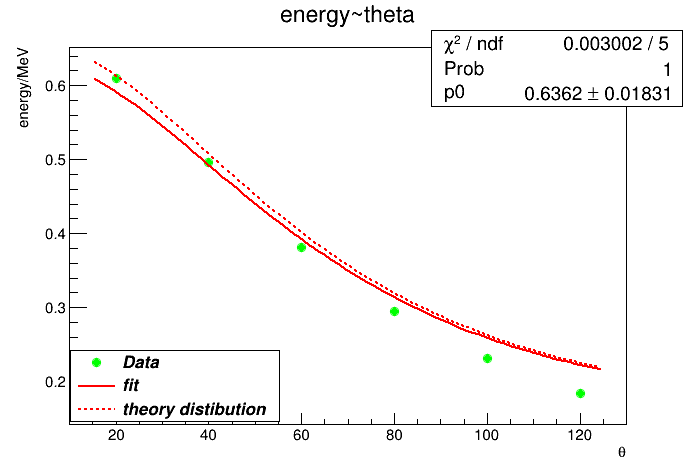
\includegraphics[width=0.7\textwidth]{data/scatterPhoton.png}
    \caption{散射光子和角度之间的关系}
    \label{fig:thetaEnergy}
\end{figure}
\subsection{散射微分截面}
选择$60^\circ$作为参考点,画出相对散射微分截面与角度之间的关系,如图~\ref{fig:fit}中对散射微分截面进行拟合
\begin{figure}[htbp]
    \centering
    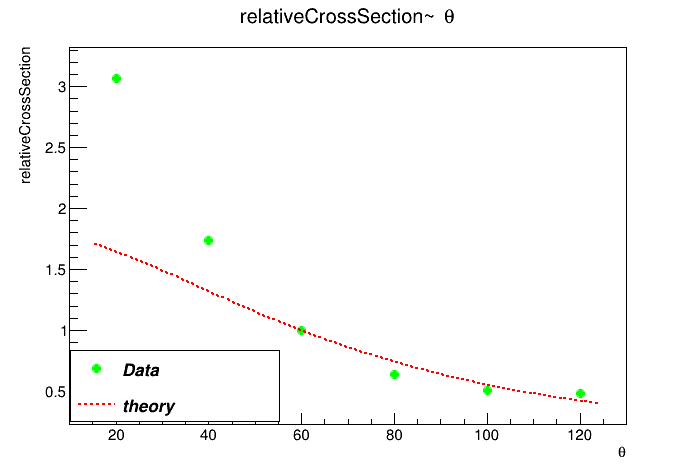
\includegraphics[width=\textwidth]{data/scatterPBarn.png}
    \caption{相对微分散射截面}
    \label{fig:fit}
\end{figure}
本文采用另外一种拟合方法\texttt{likelihood}方法将偶然符合计数和
衰变寿命同时拟合出来。
\[\tau=8.229ns\]
\[n_{rc}=0\]
\section{结论}
本实验最终给出原子核衰变寿命为$\tau=8.229ns$。
\bibliography{report}
\end{document}